%version of 01-02-19

\chapter{RECURRENCES}
\label{ch:Recurrences}

One of the intellectually most powerful strategies for all manner of
human endeavor is to ``learn from the past''---i.e., to {\em re}-use
knowledge that one has acquired earlier in order to acquire new
knowledge.  Within the domain of computing, this strategy is
exemplified by computations that derive the value of a function $F$ at
an argument $n \in \N^+$ by invoking the (hopefully, earlier-computed)
values of $F$ at arguments $1, 2, \ldots, n-1$.  The classical first
example of such a {\it recurrent} mode of computing involves the {\it
  factorial function} {\sc Fact} of Section~\ref{sec:unary-ops}.C.
\index{arithmetic!basic operations!factorial (of a nonnegative integer)}
The ``direct'' mode of computing {\sc Fact} at an argument $n \in
\N^+$ is:
\[ \mbox{\sc Fact}(n) \ = \ 1 \times 2 \times \cdots \times n. \]
The {\em recurrent} mode of computing {\sc Fact}($n$) is more
compact---and it better exposes the inherent structure of the
function.
\[ \mbox{\sc Fact}(n) \ = \ \left\{
\begin{array}{cl}
 n \times \mbox{\sc Fact}(n-1) & \mbox{ if } \ n > 1 \\
 1 & \mbox{ if } \ n = 1 \\
\end{array}
\right.
\]
This chapter is devoted to deriving and solving a variety of types of
recurrences.  In common with the rest of this text, our treatment of
this subject emphasizes exploiting recurrent structure in reasoning
and analysis: increased understanding will enable improved computing.


\section{Linear Recurrences}
\label{sec:linear-recurrences}
\index{linear recurrences}

This section is devoted to the solution of {\em linear} recurrences,
as exemplified by the following function specifications.  

\begin{equation}
\label{eq:Lin-Recur:general}
F(n) \ = \ \left\{
\begin{array}{cl}
a F(n/b) + f(n) & \mbox{for } n > b \\
1 & \mbox{for } n = b
\end{array}
\right.
\end{equation}

\begin{equation}
\label{eq:Lin-Recur:basic}
F(n) \ = \ \left\{
\begin{array}{cl}
a F(n/b) + c & \mbox{for } n \geq b \\
c & \mbox{for } n < b
\end{array}
\right.
\end{equation}

Myriad basic algorithmic problems, including sorting, selection,
matching, etc., can be solved using linear-recurrent algorithms
\cite{CLRS}---and such algorithms yield to specification and analysis
via linear recurrences.

In the next two subsections, we present analyses of recurrences
(\ref{eq:Lin-Recur:general}) and (\ref{eq:Lin-Recur:basic}).  The
reader will be able to extend the techniques we use in our analyses of
these specific recurrences in order to analyze other members of the
important family of linear-recurrent algorithms.


\subsection{The Simple Recurrence (\ref{eq:Lin-Recur:basic})} 
\label{sec:masterTheorem}
\label{sec:linear-recurrence-basic}

We focus first on the simpler of our sample recurrences, namely,
(\ref{eq:Lin-Recur:basic}).  Happily, there is a single perspicuous
proof that elegantly solves recurrences of this form.

By the time the reader has reached this paragraph, she has the
mathematical tools necessary to prove and apply what is called {\it
  The Master Theorem for Linear Recurrences} \cite{CLRS}.  The main
tools in the proof of the Theorem are: summing geometric summations
(Section~\ref{sec:geometric-sums}) and employing elementary asymptotic
notions and notations (Section~\ref{sec:asymptotics}).

\begin{theorem}[The Master Theorem for Linear Recurrences]
\label{thm:master-thm}
\index{The Master Theorem for Linear Recurrences}
Let the function $F$ be specified by the linear recurrence
(\ref{eq:Lin-Recur:basic}).  Then the value of $F$ on any argument $n$
is given by
\begin{equation}
\label{eq:Lin-Recur:solve}
\begin{array}{lcllll}
F(n) & = & (1 + \log_b n)c &  &  & \mbox{if } a=1 \\
     &   &                 &  &  & \\
     & = &
  {\displaystyle
  \frac{1-a^{\log_b n}}{1-a} \ \approx \ \frac{1}{1-a}
  }
                           &  &  & \mbox{if } a<1 \\
    &   &                  &  &  & \\
    & = &
  {\displaystyle
\frac{a^{\log_b n} -1}{a-1}
  }
                           &  &  & \mbox{if } a>1
\end{array}
\end{equation}
\end{theorem}

\begin{proof}
We expose the pattern generated by recurrence
(\ref{eq:Lin-Recur:basic}), by beginning to ``expand'' the specified
computation---replacing occurrences of $F(\bullet)$ as mandated in
(\ref{eq:Lin-Recur:basic}).  Once we discern the pattern, we jump to
the general form.
\begin{equation}
\label{eq:Lin-Recur:expand}
\begin{array}{lcccc}
F(n) & = & a F(n/b) + c & & \\
     & = & a \left( a F(n/b^2) + c \right) + c
             & = & a^2 F(n/b^2) + (a+1)c \\
     & = & a^2 \left( a F(n/b^3) + c \right) + (a+1)c
             & = & a^3 F(n/b^3) + (a^2+a+1)c \\
     &   & \vdots & & \vdots \\
     & = & 
{\displaystyle
\left(a^{\log_b n} + \cdots +a^2+a+1 \right) c
} & &
\end{array}
\end{equation}
The segment of (\ref{eq:Lin-Recur:expand}) ``hidden'' by the vertical
dots betokens an induction that is left to the reader.  Equations
(\ref{eq:geom-sum:b>1}) and (\ref{eq:geom-sum:b<1}) now enable us to
demonstrate that (\ref{eq:Lin-Recur:solve}) is the asserted
case-structured solution to (\ref{eq:Lin-Recur:basic}).  \qed
\end{proof}


\subsection{The More General Recurrence (\ref{eq:Lin-Recur:general})} 
\label{sec:linear-recurrence-general}

We now progress from the simple recurrence (\ref{eq:Lin-Recur:basic}) to
the more general recurrence (\ref{eq:Lin-Recur:general}).  We simplify
our problem in two ways, in order to avoid calculational complications
(such as floors and ceilings) that can mask the principles that govern
our analysis.
\begin{enumerate}
\item
We focus on the case $f(n) = n$.

It is a triviality to generalize to the slightly more ambitious $f(n)
= \alpha n + \beta$ (i.e., to a {\em linear} function $f$), but this
exension teaches no new lessons.
\item
We assume that the argument $n$ to functions $F$ and $f$ is a power of
$b$.

Removing this assumptions would significantly complicate our
calculations, but it would not change our reasoning.
\end{enumerate}

By ``unfolding'' (\ref{eq:Lin-Recur:general}) as in
Section~\ref{sec:linear-recurrence-basic}, we expose the algebraic
pattern created by the recurrence.  As in (\ref{eq:Lin-Recur:expand}),
once we discern this pattern, we jump to the general form (whch can be
verified via indution).
\[
\begin{array}{ccccc}
F(n) & = & a F(n/b) + n & & \\
     & = & a \left( a F(n/b^2) + n/b \right) + n
             & = & a^2 F(n/b^2) + (an/b+n) \\
     & = & a^2 \left( a F(n/b^3) + n/b^2 \right) + (a/b+1)n
             & = & a^3 F(n/b^3) + (a^2/b^2+a/b+1)n \\
     &   & \vdots & & \vdots \\
    & = & 
{\displaystyle
\left(a^{\log_b n} F(1) + \sum_{i=0}^{\log_b (n)-1} (a/b)^i \right) n
} & &
\end{array}
\]

We thus see that solving the more general recurrence
(\ref{eq:Lin-Recur:general}) requires only augmenting the solution to
the simpler recurrence (\ref{eq:Lin-Recur:basic}) by ``appending'' to
the simple solution a geometric summation whose base is the ratio
$a/b$.  The reader can now invoke the techniques from
Section~\ref{sec:summing-geometric-series:techniques} to arrive at a a
solution to (\ref{eq:Lin-Recur:general}).

When ``doing mathematics,'' one is often interested in discovering the
{\em dominant behavior} of the function $F(n)$ specified via a
recurrence such as (\ref{eq:Lin-Recur:general}).  An important lesson
to garner from the analysis we have been performing throughout this
section is the following:
\begin{itemize}
\item
When $a > b$, the behavior of $F(n)$ is dominated by the first
solution term
\[ a^{\log_b n} \cdot n \cdot  F(1) \ \ = \ \ n^{1 + \log_b a} \cdot F(1) \]
\item
When $a < b$, the behavior of $F(n)$ is dominated by the second
solution term
\begin{eqnarray*}
n \cdot \sum_{i=0}^{\log_b (n)-1} (a/b)^i
  & = &
\left( 1 \ - \  (a/b)^{\log_b (n)} \right) n \\
  & = &
n \ - \ a^{\log_b n} \\
  & = &
n \ - \ n^{\log_b a}
\end{eqnarray*}
\end{itemize}

One can learn yet more lessons about $F(n)$, specifically about how to
compute $F(n)$ (exactly or approximately) by observing the graphical
depiction in Fig.~\ref{fig:masterTheorem} of the calculation described
by recurrence (\ref{eq:Lin-Recur:general}).
\begin{figure}[htb]
\begin{center}
       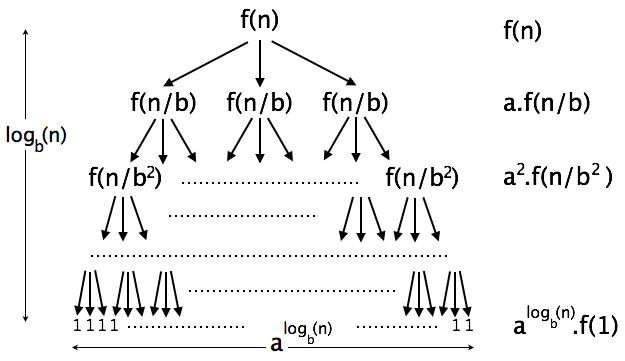
\includegraphics[scale=0.4]{FiguresMaths/MasterTheoremgeneral}
\caption{Development of the calculation specified by recurrence
  (\ref{eq:Lin-Recur:general}).  The associated summation appears on
  the right.
\label{fig:masterTheorem}}
\end{center}
\end{figure}
In particular, one observes in the figure that the computation---and
its associated tree---are perfectly balanced when $a=b$.  In
particular, when $a=b=2$, we obtain $F(n) = n \log_2(n)$.

{\Arny The notation in Fig.~\ref{fig:masterTheorem} (fonts, cdots)
  should be made consistent with the text.}


\section{Bilinear Recurrences}
\label{sec:bilinear-recurrences}
\index{bilinear recurrences}

\subsection{Binomial Coefficients and Pascal's Triangle}
\label{sec:binomial-coeff+Pascal}

In Section~\ref{sec:binomial-coeff}.C, we introduced and briefly
discussed the binomial coefficient \index{binomial coefficients}
$\displaystyle \Delta_{n,k} \ \eqdef \ {n \choose k}$ in its guise as a
binary operation on integers; see (\ref{eq:binom-coeff}).  And, we
established in Proposition~\ref{thm:manipulate-binom-coeff} the
summation rule
\[ {n \choose k} \ + \ {n \choose {k+1}} \ = \ {{n+1} \choose {k+1}} \]
for $\Delta_{n,k}$.  In fact, one can {\em define} binomial
coefficient via the {\em bilinear recurrence} that underlies this
rule.  This change in viewpoint is the topic of the current
subsection.

\subsubsection{The formation rule for Pascal's Triangle}
\label{sec:Pascal-formation}

Let us define the bivariate integer function\footnote{We alter our
  notation for binomial coefficients in deference to our change in
  viewpoint: We promote the integer pair $\langle n,k \rangle$ from a
  subscript to an argument, and we embellish $\Delta$ with a
  hat.}~$\hat{\Delta}(n,k)$ via the bilinear recurrence
\begin{equation}
\label{eq:binom-coeff-recurrence}
\hat{\Delta}(n,k) \ = \ 
\left\{
\begin{array}{cl}
1  & \mbox{ if } \ [n=1, k=0] \\
1  & \mbox{ if } \ [n=1, k=1] \\
\hat{\Delta}(n-1, k-1) \ + \  \hat{\Delta}(n-1,k) & \mbox{ otherwise}
\end{array}
\right.
\end{equation}

\smallskip

We claim that the function $\hat{\Delta}(n,k)$ thus defined is, in
fact, the for binomial coefficient $\displaystyle {n \choose k}$.  We
establish this claim with the help of a two-dimensional array of
integers known as {\it Pascal's Triangle},
\index{Pascal's triangle}
so named in honor of the French polymath Blaise Pascal.
\index{Pascal, Blaise}
Fig.~\ref{fig:pascal-triangle} provides a ``prefix'' of this famed
array, for $n,k \leq 5$.
\begin{figure}[htb]
\[
\begin{array}{c||r|r|r|r|r|r|r|r|r|r|r}
{\displaystyle {n \choose k}} & k=0 & k=1 & k=2 & k=3 & k=4 & k=5 &
k=6 & k=7 & k=8 & k=9 & \ldots \\
\hline
\hline
n=1 & 1 & 1 &    &    &     &     &    &    &   &   & \ldots \\
\hline
n=2 & 1 & 2 &  1 &    &     &     &    &    &   &   & \ldots \\
\hline
n=3 & 1 & 3 &  3 &  1 &     &     &    &    &   &   & \ldots \\
\hline
n=4 & 1 & 4 &  6 &  4 &   1 &     &    &    &   &   & \ldots \\
\hline
n=5 & 1 & 5 & 10 & 10 &   5 &   1 &    &    &   &   & \ldots \\
\hline
n=6 & 1 & 6 & 15 & 20 &  15 &   6 &  1 &    &   &   & \ldots \\
\hline
n=7 & 1 & 7 & 21 & 35 &  35 &  21 &  7 &  1 &   &   & \ldots \\
\hline
n=8 & 1 & 8 & 28 & 56 &  70 &  56 & 28 &  8 & 1 &   & \ldots \\
\hline
n=9 & 1 & 9 & 36 & 84 & 126 & 126 & 84 & 36 & 9 & 1 & \ldots \\
\hline
\vdots &\vdots &\vdots &\vdots &\vdots &\vdots &\vdots &\vdots &\vdots
&\vdots &\vdots &\ddots
\end{array}
\] 
\caption{A ``prefix'' of Pascal's Triangle, for $n,k \leq 9$.}
\label{fig:pascal-triangle}
\end{figure}
The {\em formation rule of the array} is that the array-entry at (row
$n+1$, column $k+1$) is the sum of the array-entries at (row $n$, column
$k$) and at (row $n$, column $k+1$).
\index{Pascal's Triangle!formation rule}

\medskip

By comparing the formation rule for Pascal's Triangle with equation
(\ref{eq:add-binom-coeff}), you can anticipate the following result.

\begin{prop}
\label{thm:pascal-binom}
The entries of Pascal's Triangle are the binomial coefficients.
Specifically, for all $n,k$, the entry at (row $n$, column $k$) of the
Triangle is $\displaystyle {n \choose k}$.
\end{prop}

\begin{proof}
We note by observation and direct calculation (see
Fig.~\ref{fig:pascal-triangle}) that the proposition is true for $n =
1$ and $k \in \{0, 1\}$.  A simple double induction verifies that
every binomial coefficient appears in the Triangle and every Triangle
entry is a binomial coefficient.  \qed
\end{proof}

****************** \\
induction on $n$, then for each value of $n$ on $k \leq n$ \\
{\Arny SHOULD WE SPELL THIS OUT IN DETAIL?  GIVE AS AN EXERCISE?} \\
******************

As an immediate consequence of the relation between binomial
coefficients and Pascal's Triangle, we observe the following {\it a
  priori} nonobvious fact.

\begin{prop}
\label{thm:binomcoeff-integer}
Every binomial coefficient is an integer.
\end{prop}
\index{binomial coefficients!integer-hood}

\begin{proof}
By the formation rule for Pascal's Triangle, every entry in that array
is obtained from integers via repeated additions.  The present result
therefore follows from Proposition~\ref{thm:pascal-binom}'s proof that
the elements of the Triangle are precisely the binomial coefficients.  \qed
\end{proof}


\subsubsection{The summation formula for binomial coefficients}
\label{sec:summaion-BinCoeff}

We conclude this section with a very consequential result about the
binomial coefficients.  We shall observe applications of this result
as we explore a variety of topics, ranging from counting discrete
structures and calculating probabilities to deriving basic properties
of other recursively defined families.


\begin{prop}
\label{thm:sumsof-binomcoeff}
For every positive integer $n$,
\[
\sum_{i=0}^n \ {n \choose i} \ \ = \ \
{n \choose 0} \ + \ {n \choose 1} \ + \cdots + \ {n \choose {n-1}} \ +
\ {n \choose n} \ \ = \ \ 2^n
\]
\end{prop}
\index{binomial coefficients!summation formula}

\begin{proof}
This result is an immediate consequence of the Binomial Theorem
(Theorem~\ref{thm:Binomial-theorem}).  That seminal result tells us
that, for all $n \in \N$,
\[
(x+y)^n \ \ = \ \ \sum_{i=0}^n \ \ {n \choose i} x^{n-i} y^i.
\]
If we instantiate this polynomial equation with the values $x = y =
1$, then we obtain the present result.
\qed
\end{proof}


\subsection{The Fibonacci Sequence}
\label{sec:Fibonacci}
\index{Fibonacci sequence}
\index{Fibonacci numbers}

This section is devoted to one of the most storied topics in the world
of mathematics---in terms of the topic's manifestation in the real
world and in terms of the multiple names used to refer to its
discoverer,\footnote{Not surprisingly, this marvelous sequence was
  discovered many times, in many places.  Our story refers ony to its
  discovery in the West.}~the 13th-century Italian mathematician
variously known as: \index{Fibonacci, Leonardo}
\index{Fibonacci, Leonardo!alternative names}

\begin{tabular}{ll}
Fibonacci               & (Italian for: son of Bonaccio) \\
Leonardo of Pisa        & (his hometown) \\
Leonardo Pisano         & (variant of ``of Pisa'') \\
Leonardo Pisano Bigolo  & (his hometown plus family name) \\
Leonardo Fibonacci      & (for: son of Bonaccio Bigolo) \\
Leonardo Bonacci        & (for: son of Bonaccio Bigolo) \\
\end{tabular}

\medskip

\noindent
The sequence discovered by this multi-named genius is defined as follows.

\medskip

The {\it Fibonacci sequence}, or, {\it the Fibonacci numbers}, is an
infinite sequence
\[ F(0), \ F(1), \ F(2), \ \ldots \]
of elements of $\N^+$, the set of positive integers.  As just denoted,
we see that the numbers in the sequence are traditionally indexed by
elements of $\N$, the set of nonnegative integers and are often
written using functional ($F(i)$) notation rather than subscripts
($F_i$).  The classical definition of the sequence is as follows.
\index{Fibonacci sequence!definition}\index{Fibonacci numbers!definition}
\begin{eqnarray}
\nonumber
F(0) & = & 1 \\
\label{eq:Fibonacci-defn}
F(1) & = & 1 \\
\nonumber
F(n) & = & F(n-1) \ + \ F(n-2) \ \ \ \mbox{ for all } n > 1
\end{eqnarray}
The sequence is often specified just by listing its early elements:
\[ 1, \ 1, \ 2, \ 3, \ 5, \ 8, \ 13, \ 21, \ 34, \ \ldots \]


\subsubsection{The story of the Fibonacci numbers}
\label{sec:Fibonacci-story}
\index{Fibonacci sequence!story}
\index{Fibonacci numbers!story}

Leonardo Fibonnaci describes\footnote{In his {\it Liber Abaci}}
discovering his eponymous sequence in the course of contemplating the
rate of population growth of successive generations of an idealized
immortal initial pair of rabbits.  Rabbits mature quickly and, after
attaining maturity at one month, can spawn a new pair of progeny every
following month.  So, at ``time $0$'', there is one pair of rabbits.
This persists at month $1$, because there has not yet been time to
produce new rabbits.  By month $2$, though, there are $2$ pairs of
rabbits.  At month $3$, only the first pair will have spawned, so
there are $3$ pairs of rabbits.  At month $4$, these $3$ pairs are
joined by $2$ more.  The reader can continue this story and discover
that the number of pairs of rabbits observed after successive months
are given by the sequence generated by the process implicit in
recurrence (\ref{eq:Fibonacci-defn}) and illustrated by our initial list.
Fig.~\ref{fig:fibo5} below illustrates the process up to month $4$.
\begin{figure}[htb]
\begin{center}
        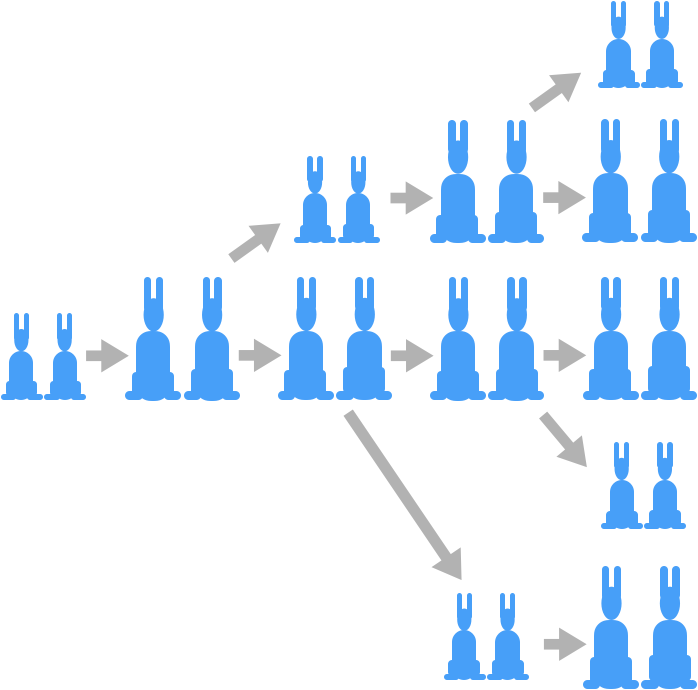
\includegraphics[scale=0.3]{FiguresMaths//Fibo5}
\caption{The successive generations of rabbits are growing each month (depicted for the $4$ first months).}
        \label{fig:fibo5}
\end{center}
\end{figure}

The Fibonacci sequence's role in describing idealized rabbit
population statistics is no more fascinating than its appearance
elsewhere in the natural world---in structural features such as the
patterns of seeds in flower heads, the numbers of petals of flowers,
the growth patterns of pine cones and pineapples, and on and on; see
\cite{Basin63}.

The story of this fascinating sequence of numbers has a macroscopic
aspect also.  Many cultures, the ancient Greeks among them, have
attributed mystical properties to (classes of) numbers; our
discussions about the {\it prime numbers} in Section~\ref{sec:primes}
and about the {\it perfect numbers} in
Section~\ref{sec:perfect-numbers+Mersenne-primes} bear witness to this
phenomenon.  One specific number that has attracted such attention is
the {\it golden ratio}, an irrational number which is usually denoted
$\Phi$ and which has the following (exact and approximate) values:
\index{golden ratio, $\Phi$}
\index{$\Phi$, the golden ratio}
\[ \Phi \ = \ \frac{1+\sqrt{5}}{2} \ \approx \  1.618\ldots \]
It has been alleged that rectangles whose {\it aspect ratios} (Length
$\div$ Width) are (roughly) $\Phi$ are the most pleasing to the human
eye.  In fact, the aspect ratio of the Parthenon, in Athens is
(roughly) $\Phi$, although it is not known whether this is
intentional.  The relevance of $\Phi$ to this section resides in the
fact that {\em the sequence of ratios of successive Fibonacci numbers
approaches $\Phi$}.

You can perform your own test about pleasing rectangles and ratios of
successive Fibonacci numbers by perusing Fig.~\ref{fig:fibosquare}.
\begin{figure}[htb]
\begin{center}
        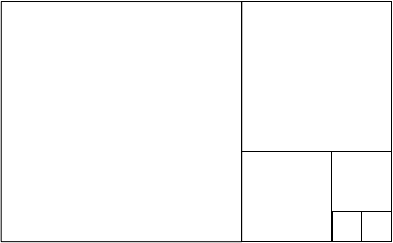
\includegraphics[scale=0.5]{FiguresMaths//Fiboembedded}
\caption{Successive Fibonacci numbers interpreted geometrically, via a
  spiral of rectangles whose respective lengths form a Fibonacci
  sequence.}
        \label{fig:fibosquare}
\end{center}
\end{figure}

The mathematical properties of this truly remarkable sequence will
occupy our attention in the remainder of this section.


\subsubsection{Fibonacci numbers and binomial coefficients}
\label{sec:FibNo+BinomCoeff}
\index{Fibonacci numbers!connection with binomial coefficients}
\index{binomial coefficients!connection with Fibonacci numbers}

%\begin{figure}[h]
%\begin{center}
%        \includegraphics[scale=0.4]{FIGmaths/DefFibo}
%        \caption{Principle of the Fibonacci progression}
%        \label{doublesum}
%\end{center}
%\end{figure}
%Notice that it is a special case of $u_{n+1} =\alpha.u_{n} + \beta.u_{n-1}$ for $\alpha=\beta=1$.
%\bigskip

There is a strong, nonobvious, connection between the binomial
coefficients of Section~\ref{sec:binomial-coeff+Pascal} and the
Fibonacci numbers of the current section.  We observe this connection
by contemplating the diagonals of Pascal's Triangle.  See
Fig.~\ref{fig:FiboPascal}.
\begin{figure}[htb]
\begin{center}
        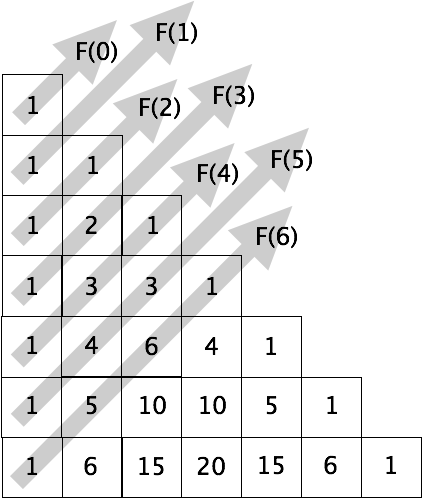
\includegraphics[scale=0.3]{FiguresMaths//FiboPascal1}
\caption{Obtaining Fibonacci numbers as diagonals of the left-justified Pascal Triangle.}
\label{fig:FiboPascal}
\end{center}
\end{figure}

\begin{prop}
\label{thm:FibNo+BinomCoeff}
For all $n \in \N$, the Fibonacci number $F(n)$ is the sum of the
first $\lceil (n+1)/2 \rceil$ binomial coefficients $\displaystyle {k
  \choose i}$ such that $k+i = n$.  Symbolically,
\begin{equation}
\label{eq:FibNo+BinomCoeff}
F(n) \ = \ {n \choose 0} \ + \ {{n-1} \choose 1} \ + \cdots + \ 
{{\lfloor (n+1)/2 \rfloor} \choose {\lceil (n+1)/2 \rceil -1}}.
\end{equation}
\end{prop}

\begin{figure}[htb]
\begin{center}
        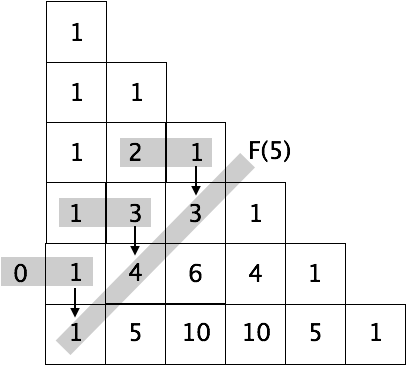
\includegraphics[scale=0.3]{FiguresMaths//FiboPascal2}
\caption{Each term of the diagonal is obtained by summing the two preceding ones.}
        \label{fig:FiboPascalExplanation}
\end{center}
\end{figure}

\begin{proof}[Sketch]
Because of the heavy calculational content of a complete proof, we
provide here just a short sketch.

Fig.~\ref{fig:FiboPascalExplanation} depicts a portion of Pascal's
Triangle with shaded diagonal and horizontal annotations.  The shaded
diagonal annotation depicts the three numbers in the Triangle that
sum to the Fibonnaci number $F(5)$.
\begin{enumerate}
\item
Looking at the three horizontal shaded areas {\em individually}
illustrates how each of the three numbers on the shaded diagonal,
being a binomial coefficient, arises as a sum of two numbers on the
preceding rowof the array---as instantiations of the formation rule
for Pascal's Triangle.  The illustrated instance of the rule asserts
that:
\[
\begin{array}{ccccccc}
{\displaystyle {5 \choose 0}}
 & = &
{\displaystyle 0 + {4 \choose 0} }
 & = &
0 + 1
 & = & 1 \\ \\
{\displaystyle {4 \choose 1}}
 & = &
{\displaystyle {3 \choose 0} + {3 \choose 1} }
 & = &
1 + 3
 & = & 4 \\ \\
{\displaystyle {3 \choose 2}}
 & = &
{\displaystyle {2 \choose 1} + {2 \choose 2} }
 & = &
2 + 1
 & = & 3
\end{array}
\]
\item
Looking at the three horizontal shaded areas {\em in tandem}
illustrates that the numbers along the shaded diagonal are sums of the
numbers along the two diagonals that are above the shaded one---as
instantiations of the formation rule for Fibonnaci numbers.  The
illustrated instance of the rule asserts that
\[ F(5) \ = \ F(4) + F(3) \ = \ 5 + 3 \ = \ 8. \]
\end{enumerate}

The preceding reasoning provides the infrastructure of an induction
that will prove that the proposition holds for every Fibonacci
number.  As suggested by the statement of the proposition, the
required calculations on indices can obscure the rather elegant basis
for the result.
\qed
\end{proof}

%Another way to write this relation is by the following expression:
%$F_n = binomial (n,0,1 ...)$


\subsubsection{Alternative generating recurrences for the Fibonacci sequence}
\label{sec:Fibonacci-other-recurrences}
\index{Fibonacci sequence!other generating recurrences}
\index{Fibonacci numbers!other generating recurrences}

Although the classical recurrence (\ref{eq:Fibonacci-defn}) is the
structurally simplest generator of the Fibonacci sequence, there exist
other generators that are not much more complex.  We now present two
other multi-linear recurrences that generate the sequence, in addition
to a family of binary generating recurrences.

\paragraph{\small\sf A. Two multi-linear generating recurrences}

\begin{prop}
\label{thm:FiboSum-1}
For all integers $n \geq 2$,
\begin{eqnarray}
\label{eq:multilinear-Fib-1}
F(n) & = &
1 \ + \ F(0) \ + \ F(1) \ + \ F(2) \ + \cdots + \ F(n-2) \\
\nonumber
     & = &
1 \ + \ \sum_{k=0}^{n-2} F(k)
\end{eqnarray}
\end{prop}

\begin{proof}
We proceed by induction.

\noindent
The {\em base case}, $n=2$, holds because $F(2) = 2 =  1 + F(0)$.

\noindent 
Assume, {\em for induction}, that 
(\ref{eq:multilinear-Fib-1}) holds for all arguments $2 \leq n < m$.

\noindent
We {\em extend} the induction as follows.  Our inductive hypothesis
assures us that for all $m \geq 3$,
\[ F(m-1) \ = \ 1 \ + \ F(0) \ + \ F(1) \ + \ F(2) \ + \cdots + \ F(m-3). \]
Combining this with the classical recurrence
(\ref{eq:Fibonacci-defn}), we therefore have
\begin{eqnarray*}
F(m) & = & F(m-2) \ + \ F(m-1) \\
     & = &
F(m-2) \ + \ 1 \ + \ F(0) \ + \ F(1) \ + \ F(2) \ + \cdots + \ F(m-3)
\end{eqnarray*}

\noindent
This extends the induction and completes the proof.
\qed
\end{proof}

\medskip

While recurrence (\ref{eq:multilinear-Fib-1}) in
Proposition~\ref{eq:multilinear-Fib-1} employs all of the Fibonnaci
numbers up to the desired bound, recurrence
(\ref{eq:multilinear-Fib-2}) in the next proposition employs only
every other such number.

\begin{prop}
\label{thm:FiboSum-2}
For all integers $n \geq 2$,
\begin{eqnarray}
\label{eq:multilinear-Fib-2}
F(n) & = &
F(n-1) \ + \ F(n-3) \ + \ F(n-5) \ + \cdots + \ C(n) \\
\nonumber
\mbox{where} &   & \\
\nonumber
C(n) & = & \left\{
\begin{array}{cl}
F(2) + F(1) = 3  & \mbox{\rm if } \ n \ \mbox{\rm is even} \\
F(1) + F(0) = 2  & \mbox{\rm if } \ n \ \mbox{\rm is odd}
\end{array}
\right.
\end{eqnarray}
We thereby sum every other term up to the $(n-1)$th and use a
``clean-up'' term $C(n)$ to complete the sum.
\end{prop}

\begin{proof}
We develop the claimed summation (\ref{eq:multilinear-Fib-2}) by
iteratively expanding the righthand term ($F(n-2)$) of the classical
recurrence (\ref{eq:Fibonacci-defn}).  This expansion begins
\begin{eqnarray}
\label{eq:multilinear-Fib-3}
F(n)
& = &
F(n-1) \ + \ F(n-2) \\
\nonumber
& = &
F(n-1) \ + \ F(n-3) \ + \ F(n-4) \\
\nonumber
& = &
F(n-1) \ + \ F(n-3) \ + \ F(n-5) \ + \ F(n-6)
\end{eqnarray}
We continue this expansion process as long as we can, and then we add
a single {\em clean-up term}, which we have designated $C(n)$ in the
statement of the proposition.

Determining the value of $C(n)$ is facilitated by noticing that our
expansion is ``trying'' to have all term-indices in the expanded
summation have the same parity.  To wit, the successive indices of the
expanded summation differ by $2$, beginning with $n-1$, $n-3$, $n-5$,
and so on; therefore, the index $n-k$ that we expand always has the
same parity as $n$.  Let us observe the consequence of this fact for
the ``end game'' of the expanson process.
\begin{itemize}
\item
When $n$ is even, our expansion eventually comes down to
\[ \begin{array}{cl}
  & \cdots + F(5) \ + \ F(4) \\
\longrightarrow 
  & \cdots + F(5) \ + \ F(2) \ + \ F(1) \\
\end{array}
\]
The expansion must end at this point because we have run out of
Fibonacci numbers!  We therefore have
\[ C(n) \ = \ F(2) \ + \ F(1) \ = \ 2 + 1 \ = \ 3. \]

\item
When $n$ is odd, our expansion eventually comes down to
\[ \begin{array}{cl}
  & \cdots + F(4) \ + \ F(3) \\
\longrightarrow
  & \cdots + F(4) \ + \ F(1) \ + \ F(0)
\end{array}
\]
The expansion must end at this point because we have run out of
Fibonacci numbers!  We therefore have
\[ C(n) \ = \ F(1) \ + \ F(0) \ = \ 1 + 1 \ = \ 2. \]
\end{itemize}
In either case, our expanded summation produces the correct value of
$F(n)$.  \qed
\end{proof}


\paragraph{\small\sf B. A family of binary generating recurrences}

What we have earlier called ``generating recurrences'' or ``formation
rules'' for binomial coefficients and Fibonacci numbers can also be
viewed as (mathematical) identities on the quantities of interest.  In
our usage, the line between ``generating recurrences'' and
``identities'' centers on computational issues: multilinear
recurrences can feasibly be used to generate the desired numbers;
nonlinear recurrences such as we expose in this subsection will likely
not be used as generators.  Indeed, for several of the results we
cover here, it is the methodology of proof and analysis that we wish
to stress.

\begin{prop}
\label{thm:Fib-higher-indices}
For all $n \in \N$ and $k < n$
\begin{equation}
\label{eq:Fib-higher-indices}
F(n) \ = \ F(k) \cdot F(n-k) \ + \ F(k-1) \cdot F(n-k-1).
\end{equation}
\end{prop}

Of course, the classical recurrence (\ref{eq:Fibonacci-defn}) is
instance $(k = 1)$ of the family of recurrent equations
(\ref{eq:Fib-higher-indices}).

\begin{proof}
We first explain how one might guess at the existence of the family of
recurrences (\ref{eq:Fib-higher-indices}), and then we validate the
recurrences in the family.

We begin with the classical recurrence (\ref{eq:Fibonacci-defn})
and iteratively use this recurrence to ``expand'' the classical
recurrence.  In detail, we begin by combining the first two instances
of (\ref{eq:Fibonacci-defn}), namely,
\[
\begin{array}{lcrrr}
F(n)   & = & F(n-1) & + & F(n-2) \\
F(n-1) & = & F(n-2) & + & F(n-3)
\end{array}
\]
and we combine them algebraically to produce the following.
\[ F(n) \ = \ 2 F(n-2) \ + \ F(n-3). \]
And then we iterate!  The following table illustrates the result of
the first four iterations of the process.
\[
\begin{array}{ccrcrcrcrcrcr}
F(n) & = & F(n) & + & F(n-1) \\
     & = &      &   & 2 F(n-1) & + & F(n-2) \\
     & = &      &   &          &   & 3 F(n-2) & + & 2 F(n-3) \\
     & = &      &   &          &   &          &   & 5 F(n-3) & + & 3 F(n-4)  \\
     & = &      &   &          &   &          &   &          & + & 8
F(n-4) & + & 5 F(n-5)  \\
 & \vdots  &  & \vdots  &  &  \vdots &  & \vdots
 &  & \vdots  &   & \vdots  & 
\end{array}
\]
Note that the coefficients of the successive occurrences of the
Fibonacci numbers $F(i)$ that occur in our table are themselves
Fibonacci numbers.  By analyzing the emerging pattern---{\em remember
  our advice in Chapter~\ref{ch:doingmath} to always look for
  patterns}---we arrive at the family (\ref{eq:Fib-higher-indices})
of recurrent equations.

{\em Keep in mind that, at this point, we are still in the realm of
  conjecture!  We must now verify the universal validity of the
  family.}

We proceed by induction on the number $k$ of iterated expansions of
the classical recurrence (\ref{eq:Fibonacci-defn}).

The {\em basis for our induction} resides in the observation we shared
right after stating the proposition: Instance $(k = 1)$ of the posited
family of recurrent equations is just the classical recurrence
(\ref{eq:Fibonacci-defn}).

Let us assume that instance $k$ of family
(\ref{eq:Fib-higher-indices}), namely, the equation
\[ F(n) \ = \ F(k) \cdot F(n-k) \ + \ F(k-1) \cdot F(n-k-1) \]
is valid, and let us observe the result of producing instance $k+1$
from this instance.  We algebraically combine the just-cited equation
with the following instantiation of the classical recurrence:
\[ F(n-k) \ = \ F(n-k-1) \ + \ F(n-k-2) \]
We find that
\begin{eqnarray*}
F(n) & = & F(k) \cdot F(n-k) \ + \ F(k-1) \cdot F(n-k-1) \\
     & = & F(k) \cdot \big[ F(n-k-1) \ + \ F(n-k-2) \big]  \ +
             \ F(k-1) \cdot F(n-k-1) \\
     & = & \big[ F(k) \ + \ F(k-1) \big] \cdot F(n-k-1) \ + \ F(k)
             \cdot F(n-k-2) \\
     & = & F(k+1) \cdot F(n-k-1) \ + \ F(k) \cdot F(n-k-2).
\end{eqnarray*}
The induction is thus extended, which establishes the proposition.
\qed 
\end{proof}

\subsubsection{Toward a closed form for the ``limit''  of the
  Fibonacci sequence}
\label{sec:Fib-Golden-Ratio}

In this section, we present the general methodology for determining
the close form of $F(n)$, that is an direct expression that only
depends on $n$ and not on the other terms of the sequence.  The
characteristic equation of $F(n+2) - F(n+1) - F(n) =0$ is:

$x^2 - x - 1 = 0$

Let determine its discriminant: $\Delta = 5$.
Since it is positive, this equation has two distinct roots:

$\Phi = \frac{1+\sqrt{5}}{2}$ and $\Phi' = \frac{1-\sqrt{5}}{2}$

The first one $\Phi$ is known as the \textit{golden ratio}. 

The general term $F(n)$ is equal to $a.\Phi^n + a'.\Phi'^n$ where $a$
and $a'$ are determined by two particular values $n=0$ and $n=1$:

$F(n)= \frac{1}{\sqrt{5}} ((\frac{1+\sqrt{5}}{2})^n - (\frac{1-\sqrt{5}}{2})^n)$


\subsection{$\oplus$ Relatives of Fibonacci Numbers and Binomial Coefficients}
\label{sec:Fibo-relatives}

\subsubsection{Lucas numbers}
\label{sec:Lucas-numbers}
\index{Lucas numbers}
\index{Lucas sequence}

A constant preoccupation of mathematicians is to understand why
important mathematical structures exhibit their observed properties.
A common way to seek such understanding is to perturb the definition
of the important structure and study the effects of the perturbation.
While this stratagem leads to interesting, valuable results only
sometimes, it is an invaluable tool in the hands of a gifted
mathematician.  This chapter is devoted to a brief survey of such a
study by the 19th-century French mathematician Fran\c{c}ois Edouard
Anatole Lucas (commonly known as Edouard Lucas).\index{Lucas, Edouard}

\paragraph{\small\sf A. Definition}

Lucas, who is credited with giving the name ``Fibonacci numbers'' to
the sequence discovered by Leonardo Pisano,
\index{Fibonacci numbers!origin of name}
investigated the consequences of perturbing the initial conditions,
$F(0) = F(1) = 1$, in the definition (\ref{eq:Fibonacci-defn}) of the
Fibonacci sequence.

Lucas's overall goal was simply to replace the Fibonacci sequence's
initial values $\langle 1,1 \rangle$, with the values $\langle 2,1
\rangle$.  It turns out to be much more fruitful---in terms of more
striking results and simpler proofs---to make a somewhat more drastic
perturbation:

The {\it Lucas sequence} \index{Lucas sequence!definition} is the
infinite sequence of positive integers
\[ L(-1), \ L(0), \ L(1), \ L(2), \ldots \]
generated by the recurrence
\begin{eqnarray}
\nonumber
L(-1) & = & 2 \\
\label{eq:Lucas-defn-1}
L(0) & = & 1 \\
\nonumber
L(n) & = & L(n-1) \ + \ L(n-2) \ \ \ \mbox{ for all } n \geq 1
\end{eqnarray}
Because we conventionally index sequences by {\em nonnegative}
numbers, we henceforth ignore $L(-1)$ and use the following {\em
  standard definition} of the Lucas sequence.
\begin{eqnarray}
\nonumber
L(0) & = & 1 \\
\label{eq:Lucas-defn-2}
L(1) & = & 3 \\
\nonumber
L(n) & = & L(n-1) \ + \ L(n-2) \ \ \ \mbox{ for all } n > 1
\end{eqnarray}

\medskip

The following finite sequences present the first few elements of both
the the Lucas sequence (for illustration) and the Fibonacci sequence
(for comparison).
\[
\begin{array}{r|rrrrrrrrrrr}
n: &
 0, & 1, & 2, & 3, &  4, &  5, &  6, &  7, &  8, &   9, & \ldots \\
\hline
L(n): &
 1, & 3, & 4, & 7, & 11, & 18, & 29, & 47, & 76, & 123, & \ldots \\
F(n): &
 1, & 1, & 2, & 3, &  5, &  8, & 13, & 21, & 34, &  55, & \ldots
\end{array}
\]

We begin our  brief study of the Lucas sequence by noting that just a
minor tweak converts the Fibonacci-related identity revealed in
Proposition~\ref{thm:FiboSum-1} to an identity about Lucas numbers.

\begin{prop}
\label{thm:LucasSum-1}
For all integers $n \geq 0$,
\begin{equation}
\label{eq:multilinear-Lucas-1}
L(n+2) \ = \
1 \ + \ L(-1) \ + \ L(0) \ + \ L(1) \ + \ L(2) \ + \cdots + \ L(n)
\end{equation}
\end{prop}

\begin{proof}[Sketch]
We can literally repeat the proof of Proposition~\ref{thm:FiboSum-1},
with only a change in the induction's base case, which becomes
\[ L(2) \ = \ L(-1) + L(0) + 1 \ = \ 2 + 1 + 1 \ = \ 4. \]
The body of the inductive argument holds for the Lucas sequence as
well as for the Fibonacci sequence.
\qed
\end{proof}

\paragraph{\small\sf B. Relating the Lucas and Fibonacci numbers}

There are several simple equations that relate the Lucas and Fibonacci
numbers.  We present a few of the most aestetically pleasing
ones,\footnote{Aesthetically pleasing, that is, to the authors.  As
  noted by the author Margaret Wolfe Ungerford in {\it Molly Bawn}
  (1878),\index{Ungerford, Margaret Wolfe} ``Beauty is in the eye of
  the beholder.''}~in terms of their exposing an intimate
relationship between the two sequences.
\index{Fibonacci numbers!relations with Lucas numbers}
\index{Lucas numbers!relations with Fibonacci numbers}

\begin{prop}
\label{thm:Lucas-n:2Fibs}
For all $m, n \geq 1$
\begin{eqnarray}
\label{eq:L-F-a}
\mathbf{(a) } \ \ 
L(n) & = & F(n+1) + F(n-1) \\
\label{eq:L-F-b}
\mathbf{(b) } \ \
F(n+1) & = & \frac{1}{2} \big(F(n) \ + \ L(n) \big) \\
\label{eq:L-F-c}
\mathbf{(c) } \ \
F(m + n-1) & = & \frac{1}{2} \big( F(m) \cdot L(n) \ + \ F(n) \cdot L(m) \big) \\
\label{eq:L-F-d}
\mathbf{(d) } \ \
F(2n) & = & F(n) \cdot L(n).
\end{eqnarray}
\end{prop}

\begin{proof}
We consider the three identities in turn.

\noindent {\bf (a)}
We proceed by induction.

\medskip

\noindent
{\it The base case.}
Equation (\ref{eq:L-F-a}) holds when $n=1$ because
\[ L(1) = 3 = F(2) + F(0) = 2+1. \]

\medskip

\noindent
{\it The inductive hypothesis}.
Assume that equation (\ref{eq:L-F-a}) holds for $L(2), L(3), \ldots,
L(n)$.

\medskip

\noindent
{\it The inductive extension}. 
Let us compute $L(n+1)$:
\begin{itemize}
\item
By definition (\ref{eq:Lucas-defn-2}),
\begin{equation}
\label{eq:L-FF-1}
L(n+1) \ = \L(n) \ + \ L(n-1).
\end{equation}
\item
When we apply the inductive hypothesis to both addends in
(\ref{eq:L-FF-1}), we obtain (after rearranging terms):
\begin{equation}
\label{eq:L-FF-2}
L(n+1) \ = \  F(n+1) \ + \ F(n) \ + \ F(n-1) \ + \ F(n-2)
\end{equation}
\item
Finally, we invoke the defining recurrence (\ref{eq:Fibonacci-defn})
of the Fibonacci numbers on the first two addends in (\ref{eq:L-FF-2})
and on the last two addends.  We thereby transform (\ref{eq:L-FF-2})
to equation (\ref{eq:L-F-a}), which validates the latter identity.
\end{itemize}

\[ \approx \approx \approx \approx \approx \approx \approx \approx \approx \approx \]
Notice that a proof similar to the preceding one yields the identity
$L(n) = F(n+2) + F(n-2)$.  Similar, but more complicated, identities
hold for larger arguments.  For the cases $n+3$ and $n+4$, for
instance, one can establish the following pair of identities.
\begin{eqnarray}
\label{eq:LF:n+3}
L(n) & = & \frac{1}{2} (F(n+3)+F(n-3)) \\
\label{eq:LF:n+4}
L(n) & = & \frac{1}{3} (F(n+4)+F(n-4))
\end{eqnarray}
{\Arny Perfect exercises, no?}
\[ \approx \approx \approx \approx \approx \approx \approx \approx \approx \approx \]

\bigskip

\noindent {\bf (b)}
By direct calculation, we derive the desired rsult:
\begin{eqnarray*}
2 F(n+1) & = & F(n+1) \ + \ F(n) \ + \ F(n-1) \\
         & = & L(n) \ + \ F(n).
\end{eqnarray*}

\bigskip

\noindent {\bf (c)}
This identity is verified via a somewhat complicated induction.  We
fix parameter $n$ in the argument $F(m+n)$ and induce on parameter $m$.

\medskip

\noindent
{\it The base case.}
Because $L(0) = F(0)= 1$ the instance $m=0$ of identity
(\ref{eq:L-F-c}) reduces to identity (\ref{eq:L-F-b}), which we have
just proved.  To wit,
\[ F(n+1) \ = \ \frac{1}{2} \big( L(n) \ + \ F(n) \big)
\ = \ \frac{1}{2} \big( F(0) \cdot L(n) \ + \ F(n) \cdot L(0) \big).
\]

\medskip 

\noindent
{\it The inductive hypothesis}.
Let us assume that identity (\ref{eq:L-F-c}) holds for all $m \leq k$.

\medskip

\noindent
{\it The inductive extension}.
Let us focus on instance $m = k+1$ of identity (\ref{eq:L-F-c}).  Note
first that the classical Fibonacci recurrence
(\ref{eq:Fibonacci-defn}) implies that
\[ F(n + k +1) \ = \ F(n + k) \ + \ F(n + k - 1). \]
When we apply the inductive hypothesis to both $F(n + k)$ and $F(n + k
- 1)$, we obtain the following two identities.
\begin{eqnarray*}
F(n + k) & = & \frac{1}{2} \big( F(k-1) \cdot L(n) \ + \ F(n) \cdot
L(k-1) \big) \\
F(n + k - 1) & = & \frac{1}{2} \big( F(k-2) \cdot L(n) \ + \ F(n) \cdot L(k-2) \big).
\end{eqnarray*}
Because both the Fibonacci and Lucas sequences obey the body of
recurrence (\ref{eq:Fibonacci-defn}), the preceding equations combine
to extend the induction.  To wit,
\begin{eqnarray*}
2 F(n + k +1) & = & 2 F(n + k) \ + \ 2 F(n + k - 1) \\
              & = & 
\big( F(k-1) \cdot L(n) \ + \ F(n) \cdot L(k-1) \big)
\ + \
\big( F(k-2) \cdot L(n) \ + \ F(n) \cdot L(k-2) \big) \\
              & = &
L(n) \cdot \big( F(k-1) \ + \ F(k-2) \big)
\ + \
F(n) \cdot \big( L(k-1) \ + \ L(k-2) \big) \\
              & = &
L(n) \cdot F(k) \ + \ F(n) \cdot L(k)
\end{eqnarray*}
The thus-extended induction verifies identity (\ref{eq:L-F-c}).

\bigskip

\noindent {\bf (d)}
Identity ((\ref{eq:L-F-d}) is actually the case $m=n$ of identity
((\ref{eq:L-F-c}).

This validates our final identity, which completes the proof.  \qed
\end{proof}


\subsubsection{Tree-Profile numbers}
\label{sec:Tree-Profile-numbers}
\index{Tree-Profile numbers}

In the course of analyzing a genre of search tree called {\it
  2,3-trees},\footnote{These search trees are the lowest-index
  instances of the {\it B-trees} that have proved so useful in database
  implementations \cite{CLRS}.}~in \cite{MillerPRS79,RosenbergS78}, a
new number sequence was discovered.
\index{search trees}
\index{search trees!2,3-trees}
\index{search trees!B-trees}
Named {\it Tree-Profile numbers} \cite{Rosenberg79}, this family of
positive integers was found to be a close relative of the family of
binomial coefficients, both in its defining recurrence and in the
quite similar properties that the two families share.

\paragraph{\small\sf A. Definition}
\index{tree-profile numbers}

The {\it tree-profile numbers} are a doubly-indexed family
\[ \big\{ P(n,k) \big\}_{n \geq 1; \ k \geq 0}  \]
of positive integers specified by the following recursive definition.
\index{tree-profile numbers!definition}
\begin{equation}
\label{eq:TP-defn}
\begin{array}{ccl}
P(n,0) & \equiv & 1 \ \ \ \ \ \mbox{ for all } \ n \geq 1 \\
  & & \\
P(n,1) & = &
  {\displaystyle
\left\{
\begin{array}{cl}
 1 & \mbox{ for } \ n=1 \\
 2 & \mbox{ for all } \ n > 1
\end{array}
\right.  } \\
  & & \\
P(n+1, k+1) & = & P(n,k) + 2 P(n, k-1) \ \ \  \mbox{ for all } n > 1, k > 0
\end{array}
\end{equation}
\index{tree-profile numbers!triangle of numbers}

This somewhat complicated definition can be better understood with the
help of an analogue of Pascal's Triangle that we call the {\it
  Tree-profile Triangle}.  The reader may want to comapare
Fig.~\ref{fig:pascal-triangle} with Fig.~\ref{fig:TP-triangle}.

\begin{figure}[htb]
\[
\begin{array}{c||r|r|r|r|r|r|r|r|r|r|r}
P(n, k) & k=0 & k=1 & k=2 & k=3 & k=4 & k=5 & k=6 & k=7 & k=8 & k=9 & \ldots \\
\hline
\hline
n=1 &  1 &  1 &    &    &     &     &     &     &     &     \\
\hline
n=2 &  1 &  2 &  3 &  2 &     &     &     &     &     &     \\
\hline
n=3 &  1 &  2 &  4 &  7 &   8 &   4 &     &     &     &     \\
\hline
n=4 &  1 &  2 &  4 &  8 &  15 &  22 &  20 &   8 &     &     \\
\hline
n=5 &  1 &  2 &  4 &  8 &  16 &  31 &  52 &  64 & 48  &  16 \\
\hline
n=6 &  1 &  2 &  4 &  8 &  16 &  32 &  63 & 114 & 168 & 176 \\
\hline
n=7 &  1 &  2 &  4 &  8 &  16 &  32 &  64 & 127 & 240 & 396 \\
\hline
n=8 &  1 &  2 &  4 &  8 &  16 &  32 &  64 & 128 & 255 & 494 \\
\hline
n=9 &  1 &  2 &  4 &  8 &  16 &  32 &  64 & 128 & 256 & 511 \\
\hline
\vdots &\vdots &\vdots &\vdots &\vdots &\vdots &\vdots &\vdots &\vdots
&\vdots &\vdots &\ddots
\end{array}
\] 
\caption{A ``prefix'' of the Tree-Profile Triangle, for $n,k \leq 9$.}
\label{fig:TP-triangle}
\end{figure}


\paragraph{\small\sf B. Relating Triangle-Profile numbers with binomial coefficients}
\index{tree-profile numbers!relations with binomial coefficients}

\begin{prop}
\label{thm:TP=sum-of-bincoeff}
For all $n \geq 1$ and all $k \geq 0$,
\begin{equation}
\label{eq:TP=sum-of-bincoeff}
P(n,k) \ = \ 2^{k-n} \cdot \sum_{i=0}^{2n-k} {n \choose i}
\end{equation}
\end{prop}

\begin{proof}
We proceed by induction on $n$.

\medskip

\noindent
{\it The base case.}
The case $n=1$ of (\ref{eq:TP=sum-of-bincoeff}) follows from the
``boundary cases'' of definition (\ref{eq:TP-defn}).

\medskip

\noindent
{\it The inductive hypothesis.}
Let us assume that (\ref{eq:TP=sum-of-bincoeff}) holds for all $n$ up
to (but not including) some integer $m$.  Focus on an arbitrary
Tree-Profile number $P(m,k)$.
\begin{itemize}
\item
If $k \in \{0,1\}$, then the ``boundary cases'' of definition
(\ref{eq:TP-defn}) assure us that
\[
P(m,k) \ \ = \ \ 2^k \ \ = \ \ 2^{k-n} \cdot 2^n \ \ = \ \ 
2^{k-n} \cdot \sum_{i=0}^{2n-k} {n \choose i}
\]

\item
If $k > 1$, then the defining recurrence in (\ref{eq:TP-defn})
combines with the inductive hypothesis to yield:
\begin{eqnarray*}
\nonumber
P(m, k) & = &
   P(m-1, k-1) \ + \ 2 P(m-1, k-2) \\
        & = &
   2^{k-m} \cdot \sum_{i=0}^{2m-k-2} {m-1 \choose i}
   \ + \
   2^{k-m} \cdot \sum_{j=0}^{2m-k-1} {m-1 \choose i} \\
        & = &
   2^{k-m} \cdot {m \choose 0}
   \ + \
   2^{k-m} \cdot \sum_{i=1}^{2m-k-1} {m-1 \choose i}
   \ + \
   {{m-1} \choose {i-1}} \\
        & = &
   2^{k-m} \cdot \sum_{i=0}^{2m-k-1} {m \choose i}.
\end{eqnarray*}
\end{itemize}
The induction is thus extended, thereby establishing the proposition.
\qed
\end{proof}

Proposition~\ref{thm:TP=sum-of-bincoeff} explains the proliferation of
powers of $2$ in the Tree-Profile Triangle.

\begin{corol}
For all $n > k$, $P(n,k) = 2^k$.
\end{corol}

\medskip

Finally, we derive the successor Tree-Profile values that allow us to
generate the Tree-Profile Triangle.

\begin{prop}
\label{thm:successor-TP-values}
\begin{eqnarray*}
\nonumber
\mathbf{(a)} \ \
P(n, k+1) & = & 
  2 P(n,k) - 2^{k-n+1} {n \choose {k-n+1}} \\
\label{eq:successor-TP-values}
          &   & \\
\nonumber
\mathbf{(b)} \ \
P(n+1, k) & = &
  P(n,k) + 2^{k-n-1} \left[ {n \choose {k-n}} + {{n+1} \choose {k-n}} \right]
\end{eqnarray*}
\end{prop}

\begin{proof}
The major recurrence in (\ref{eq:TP-defn}) can be decomposed into the
following triplet of recurrences.
\begin{eqnarray}
\label{eq:TP-recurrence-1}
P(n, k)   & = & P(n-1, k-1) \ + \ 2 P(n-1, k-2) \\
\label{eq:TP-recurrence-2}
P(n, k+1) & = & P(n-1, k) \ + \ 2 P(n-1, k-1) \\
\label{eq:TP-recurrence-3}
P(n+1, k) & = & P(n, k-1) \ + \ 2 P(n, k-2)
\end{eqnarray}
We use the recurrences in this triplet to attack the two alleged
recurrences in the proposition.

\medskip

\noindent {\bf (a)}
Combining recurrences (\ref{eq:TP-recurrence-1}) and
(\ref{eq:TP-recurrence-2}) leads, via
Proposition~\ref{thm:TP=sum-of-bincoeff}, to the following chain of
equalities.
\begin{eqnarray*}
P(n, k+1) \ - \ P(n, k)
  & = &
P(n-1, k) \ - \ 4 P(n-1, k-2) \\
  & = &
2^{k-n+1} \cdot \left[
\sum_{i=0}^{2n-k-3} {{n-1} \choose i} \ - \
\sum_{i=0}^{2n-k-1} {{n-1} \choose i}
\right] \\
  & = & 
- 2^{k-n+1} \cdot \left[
{{n-1} \choose {2n-k-2}} \ + \ {{n-1} \choose {2n-k-1}}
\right] \\
  & = &
- 2^{k-n+1} \cdot {n \choose k-n+1}.
\end{eqnarray*}
This chain thus yields part {\bf (a)} of the proposition.

\medskip

\noindent {\bf (b)}
This part of the proposition follows by direct calculation from
recurrence (\ref{eq:TP-recurrence-3}) and
Proposition~\ref{thm:TP=sum-of-bincoeff}.  To wit,
\begin{eqnarray*}
P(n+1, k) \ - \ P(n, k)
  & = &
P(n, k-1) \ + \ 2 P(n, k-2) \ - \ P(n,k) \\
  & = &
2^{k-n-1} \cdot \left[
\sum_{i=0}^{2n-k+1} {n \choose i}
 \ - \ \sum_{i=0}^{2n-k+2} {n \choose i}
 \ - \ 2 \sum_{i=0}^{2n-k} {n \choose i}
\right] \\
  & = & 
2^{k-n-1} \cdot \left[
  2 {n \choose {2n-k}} \ + \ {n \choose {2n-k+1}} \right] \\
  & = &
2^{k-n-1} \cdot \left[
   {n \choose {k-n}} \ + \ {{n+1} \choose {k-n}} \right]
\end{eqnarray*}
This chain thus yields part {\bf (b)} of the proposition, completing
the proof.
\qed
\end{proof}

\paragraph{\small\sf C. The summation formula for Triangle-Profile numbers}
\index{tree-profile numbers!summation formula}

We observed in Proposition~\ref{thm:sumsof-binomcoeff} that the
binomial coefficients in successive rows of Pascal's Triangle sum to
successive powers of $2$.  While not quite matching that level of
elegance, we show now that the Tree-Profile numbers in successive rows
of the Tree-Profile Triangle sum to $1$ less than successive powers of
$3$.

\begin{prop}
\label{thm:TP-summation}
For all $n \in \N^+$,
\begin{equation}
\label{eq:TP-summation}
S_n \ \ \eqdef \ \ \sum_{k=0}^{2n-1} P(n,k) \ \ = \ \ 3^n -1.
\end{equation}
\end{prop}
 
\begin{proof}
We begin with the following consequence of
Proposition~\ref{thm:TP=sum-of-bincoeff}:
\[
S(n) \ \ = \ \
  \sum_{k=0}^{2n-1} P(n,k)
     \ \ = \ \
  1 \ + \ \sum_{k=0}^{2n-1} P(n,k+1).
\]
If we now invoke Proposition~\ref{thm:successor-TP-values}(a), then we
find that
\[
S(n) \ \ = \ \ 1 \ + \ 2 \cdot \sum_{k=0}^{2n-1} 
  \big( P(n,k) \ - \ 2^{k-n} {n \choose {k-n+1}} \big).
\]

We can combine the preceding expressions with the ``restricted''
Binomial Theorem (Theorem~\ref{thm:restricted-binomial-thm}) to
generate the following chain of equalities.
\begin{eqnarray*}
S(n) & = & 
\sum_{j=0}^{2n-1} 2^{n-j} {n \choose j} \ - \ 1  \\
     & = &
2^n \cdot \sum_{j=0}^{2n-1} 2^{-j} {n \choose j} \ - \ 1 \\
     & = & 
2^n \cdot (3/2)^n \ - \ 1 \\
     & = &
3^n -1.
\end{eqnarray*}

The summation formula (\ref{eq:TP-summation}) follows.
\qed
\end{proof}


\subsection{$\oplus$ Computing Products of Consecutive Fibonacci Numbers}
\label{sec:product-Fn-Fn+1}
\index{Fibonacci numbers!product of consecutive}

One feature of the Fibonacci numbers that has captivated an entire
community of mathematically oriented people is the plethora of simply
presented identities involving the numbers.\footnote{Indeed, an entire
  research journal, {\it The Fibonacci Quartlerly},\index{The
    Fibonacci Quartlerly} is dedicated to the mathematics of Fibonacci
  numbers and their kin, including the sharing of such identities.}
We now present a particularly beautiful identity.

\begin{prop} 
\label{thm:FiboSumConsecutive}
For all $n \geq 1$,
\begin{equation}
\label{eq:FiboSumConsecutive}
F(n) \cdot F(n-1) \ \ = \ \ \sum_{k=0}^{n-1} (F(k))^2.
\end{equation}
\end{prop}

\begin{proof}
One can observe identity (\ref{eq:FiboSumConsecutive}) ``in action''
in Fig.~\ref{fig:fibosquare}.  We augment this visual validation of
the identity with the following induction.

\medskip

\noindent {\it Base case.}
Instance $n=1$ of identity (\ref{eq:FiboSumConsecutive}) is valid
because
\[ F(0) \cdot F(1) \ = \ 1 \cdot 1 \ = \ 1^2 \ = \ (F(0))^2. \]

\medskip

\noindent {\it Inductive hypothesis.}
Assume that identity (\ref{eq:FiboSumConsecutive}) is valid for all $n
\leq m$.

\medskip

\noindent {\it Inductive extension.}  Let us focus on the product
$F(m+1) \cdot F(m)$.  Invoking the defining Fibonacci recurrence
(\ref{eq:Fibonacci-defn}) and the inductive hypothesis, we generate
the following chain of identities.
\begin{eqnarray*}
F(m+1) \cdot F(m)
 & = &
   (F(m) + F(m-1)) \cdot F(m) \\
 & = &
   (F(m))^2 + \big( F(m) \cdot F(m-1) \big) \\
 & = & 
   (F(m))^2 + \big( \sum_{k=0}^{m-1} (F(k))^2 \big) \\
 & = &
   \sum_{k=0}^{m} (F(k))^2.
\end{eqnarray*}
The induction is thus extended, which completes the proof.
\qed
\end{proof}


\section{Recurrences ``in action'': The Token Game}
\label{sec:TokenGame}


**HERE

We describe the (single-player) combinatorial {\it Token Game} and use
recurrences to analyze optimal plays of the game.

\subsection{The Token Game}
\label{sec:TokenGame-Rules}

The order-$n$ version of the Token Game is played with a {\it bank}
with $n$ positions, labeled $1$, \ldots, $n$ and with a {\it pile} of
$n$ tokens; see Fig.~\ref{fig:jeujetonsInit}.  In any play of the
game, the bank is initially empty.
\begin{figure}[h]
\begin{center}
        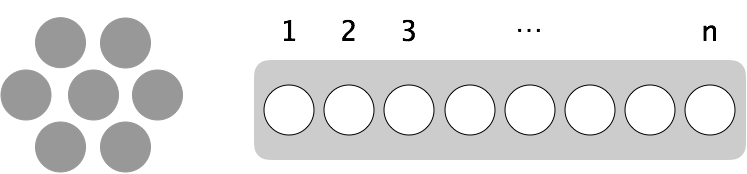
\includegraphics[scale=0.35]{FiguresMaths/GameTokenInit.png}
\caption{The initial configuration of the Token Game: Each of the $n$
  tokens appears as a grey circle, and the empty bank has $n$ slots
  where the tokens can fit.}
        \label{fig:jeujetonsInit}
\end{center}
\end{figure}
\begin{itemize}
\item
{\it Object of the game:} To fill all of the bank's slots with the $n$
tokens.

\item
{\it Each move of the game:} Move one token from the pile to the bank
{\em or} remove one token from the bank and return it to the pile.

\item
{\it Constraints of the game:} There are two rules:

\textbf{Rule 1.} If Slot \# 1 of the bank:
  \begin{itemize}
  \item
is {\em empty}, then move a token from the pile into Slot \# 1.
  \item
is {\em full}, i.e., contains a token, then remove that token from
Slot \# 1 and return it to the pile; see Fig.~\ref{fig:rule1}.
\begin{figure}[h]
\begin{center}
        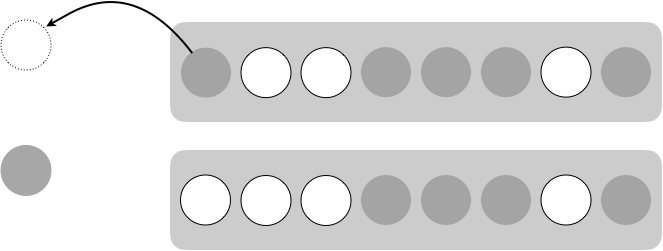
\includegraphics[scale=0.35]{FiguresMaths/GameTokenRule1.png}
\caption{Rule 1: (TOP) Slot \#1 contains a token.  (BOTTOM) Therefore,
  remove it (i.e., move it back to the pile).}
        \label{fig:rule1}
\end{center}
\end{figure}
  \end{itemize}
\textbf{Rule 2.} Focus on the bank-slot immediately to the right of
the first empty bank-slot.  If this slot
  \begin{itemize}
  \item
is {\em empty}, then move a token from the pile into Slot \# 1.
  \item
is {\em full}, i.e., contains a token, then remove that token from
Slot \#1 and return it to the pile; see Fig.~\ref{fig:rule2}.
\begin{figure}[h]
\begin{center}
        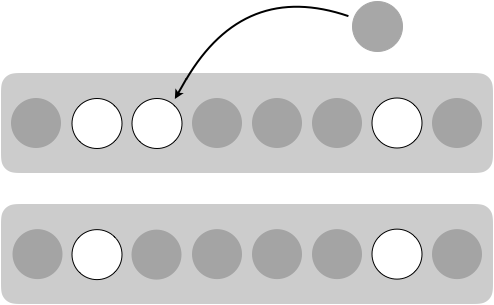
\includegraphics[scale=0.35]{FiguresMaths/GameTokenRule2.png}
\caption{Rule 2: (TOP) Slot \#$c$, which is immediately to the right
  of the first empty slot ($c=3$ in this example) is empty.  (BOTTOM)
  Therefore, move a token from the pile to Slot \#$3$.}
        \label{fig:rule2}
\end{center}
\end{figure}
  \end{itemize}

\item
{\it Objective of a play of the game:} To minimize the number of moves
from an initially empty bank to the finally full bank.
\end{itemize}

%Note that Rule 1 refers only to the slot whose full/empty status can
%change in this step, whereas Rule 2 depends on the status of slots
%whose full/empty status cannot change in this step.

\subsection{Strategies for Playing the Game}
\label{sec:Token-Game-Strategies}

The initial move of the game always involves an invocation of Rule 1,
because the bank is initially empty.  But, thereafter, one may
possibly have access to more than one move.  The question is how to
decide which move to make when one has access to more than one.

We lay the groundwork for devising an optimal strategy for playing the game
by making some observations.







The analysis of the game for some particular values of $n$ leads to some evidences (looking at the first ranks):
First, in the even case, the process should start by putting the second token while in the odd case, we should start to fill the first position.
%Then, the first token is flipped every double steps, the second one every four steps and so on.
Second observation: both rules are applied alternatively (this is obvious for Rule 1 since applying it twice consecutively leads to the initial position, 
and easy to check for Rule 2 on the first ranks). 
However, the solution is not easy to describe and its cost is not easy to establish.

The solution can be easily expressed recursively as follows (for $n > 2$):
the token in the last position can only be put bu rule 2, that means that the first $(n-2)$ one are on the bank.
Then, if we empty these first $n-2$ positions,
we obtain a configuration similar as in the initial one except for the last position which has a token. 
Then, the puzzle is solved by applying the same process on a bank with $n-1$ tokens.
The successive steps of this recursive solution are depicted in Figure~\ref{fig:jeujetonsPrinciple}.

%Thus, flipping the first tokens of the same color is different if they are all blue or red.
%Notice that flipping the first reds can be obtained using the reverse process as for the blue ones (see coding at the end of this document).

\begin{figure}[h]
\begin{center}
        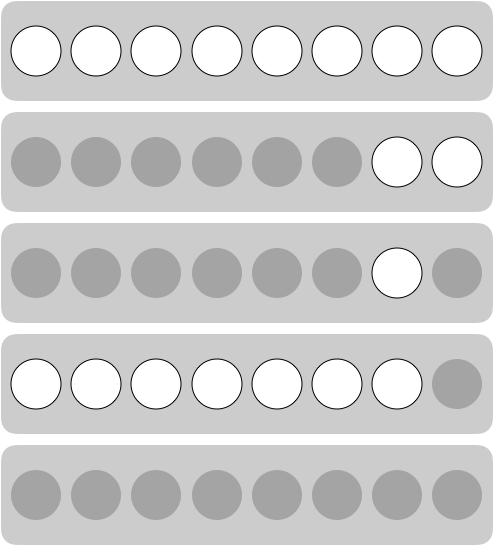
\includegraphics[scale=0.4]{FiguresMaths/GameTokenPrinciple.png}
        \caption{Principle of the recursive solution. Fill the bank in the $(n-2)$ first positions, then, put a token on the last position (Rule 2), 
        empty the (n-2) first positions. Finally, fill the $(n-1)$ first positions of the bank.}
        \label{fig:jeujetonsPrinciple}
\end{center}
\end{figure}
\bigskip

More formally,
\bigskip

fillBank(n)
\begin{itemize}
\item
 if $n=1$ then putToken(1) -- according to Rule 1
\item
if $n=2$ then PutToken(2) -- Rule 2 -- and then PutToken(1) -- Rule 1

\item 
if $n > 2$ then
\begin{itemize}
\item fillBank(n-2)
\item PutToken(n)
\item EmptyBank(n-2)
\item FillBank(n-1)
\end{itemize}
\end{itemize}

\subsection{Analysis}

The analysis comes directly from the previous process. 

Let call $f(i)$ the cost for filling the bank from position $1$ to position $i$
(the cost here refers to the number of elementary moves, put or remove a token).
Notice that it requires the same number of steps to fill or to empty the truncated bank (from position $1$ to $i$). 
The total cost is to fill the whole bank of size $n$, thus we have to solve:

$f(n) = f(n-2) + 1 + f(n-2) + f(n-1) = f(n-1) + 2.f(n-2) +1$ for $n > 2$

with $f(1) = 1$ and $f(2) = 2$.
\bigskip

If we add $f(n-1)$ in both sides of the previous expression, we obtain a simpler equation (call $s(n)$ the sum $f(n)+f(n-1)$ $n \geq 2$,
in particular, $s(2) = 2+1$):

$f(n) + f(n-1) = 2.f(n-1) + 2.f(n-2) +1$

$s(n) = 2.s(n-1)+1 = 2.(2.s(n-2)+1) + 1 = 2^2 s(n-2) + 2+ 1 = 2^3 s(n-3) + 2^2 + 2 + 1 = ... = 2^{n-2} s(2) + 2^{n-3} + ... + 2^2 + 2 + 1$ where $s(2) = 2+1$

$s(n) = 2^{n-1} + 2^{n-2} + 2^{n-3} + ... + 2^2 + 2 + 1$ 

Summing up this geometric series leads to
$s(n) = 2^{n} -1$
\bigskip

Coming back to the $f(n)$, we can rewrite this equation as:

$f(n) = 2^{n} - f(n-1) -1$ where $f(1)=1$

$f(n) = 2^{n} - 2^{n-1} + f(n-2) +1 -1 = 2^{n} - 2^{n-1} + 2^{n-2} - f(n-3) -1 = ...$

This sequence is an alternate series of the powers of $2$ where the $1$ and $-1$ are cancelled two by two.
However, there is a different number of steps if $n$ is even or not. 
In this case, the last term is $-2$, while it is $-1$ when $n$ is odd.
\bigskip

For $n$ even, $f(n) = \sum_{1 \leq k \leq n}(-1)^{k}2^{k} $

For $n$ odd, $f(n) = \sum_{0 \leq k \leq n}(-1)^{k+1}2^{k} $
\bigskip

$f(n)$ is an alternate series of the successive powers of $2$, which can be solved by a graphical proof.

We rewrite it by gathering the positive and negative terms as follows (for odd $n$): 
$f(n) = (2^{n} + 2^{n-2} + ... + 2) - (2^{n-1} + 2^{n-3} + ... + 1)$

$= 2.(2^{n-1} + 2^{n-3}  + ...  +1) - (2^{n-1} + 2^{n-3}  + ... + 1)$

$= 2^{n-1} + 2^{n-3}  + ...  +1$ 

Consider first the odd case (here, $2^{n+1}$ is a perfect square).
Figure~\ref{fig:alternatePowers2odd} gives a representation of $f(n)$ 
where the smallest surface at the right is the unit square.

Take 3 copies of $f(n)$ as it is depicted in figure~\ref{fig:alternatePowers2finalOdd},
two are mirror configurations and the third one (represented in grey) fills the remaining part of a big square but some idle space at the 2 extreme right corners. 
The whole surface is a perfect $2^{n} \times 2^{n}$ square, equal to $2^{n+1}$ plus the small surface equal to half of the basic unit square ($2 \times \frac{1}{2}$ = 1). Thus, $3.f(n)+1= 2^{n+1}$.

\begin{figure} [h]
\begin{center}
        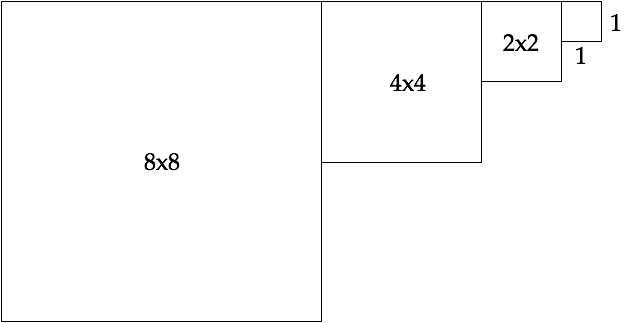
\includegraphics[scale=0.4]{FiguresMaths/alternatePowers2initOdd.png}
        \caption{Representation of the alternate series of powers of $2$ for $n=7$.
        f(7)=64+16+4+1.}
        \label{fig:alternatePowers2odd}
\end{center}
\end{figure}

\begin{figure} [h]
\begin{center}
        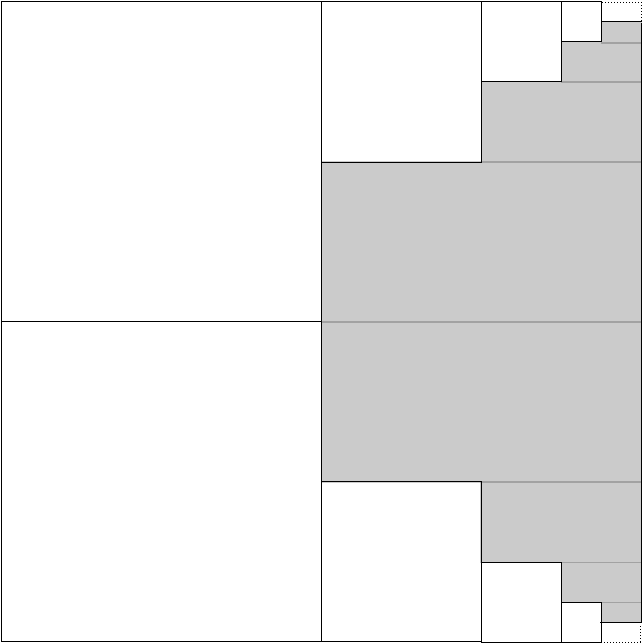
\includegraphics[scale=0.4]{FiguresMaths/alternatePowers2odd.png}
        \caption{Even case: Geometric proof using 3 copies of $f(n)$ that almost fill a large square.}
        \label{fig:alternatePowers2finalOdd}
\end{center}
\end{figure}

The previous construction may be adapted in the even case in a similar way.
The details are left to the readers. 

We propose below another proof obtained by using the results for the odd case:

We start by the expression $f(n) + f(n-1) = 2^n -1$
that is $f(2k) = 2^{2k} - f(2k-1) -1$ for even $n=2k$.

Now, apply the final expression of $f$ to $2k-1$, which is odd: $f(2k-1) = \frac{1}{3} (2^{2k+1}-1)$.

$f(2k) = 2^{2k} - \frac{1}{3} (2^{2k-1+1}-1) -1 = 2^{2k} (1-\frac{1}{3}) + \frac{1}{3} -1= \frac{1}{3} (2^{2k+1} -2)$.
\bigskip

%
%Figures~\ref{fig:alternatePowers2even} and~\ref{fig:alternatePowers2finalEven} illustrate the construction in the even case.
%The details are left to the readers. 
%We obtain $3.f(n)+2= 2^{n+1}$ by a similar analysis.
%However, we can deduce directly the even case from the odd case by remarking that $f(2k)=2.f(2k-1) +1$.
%
%This is obtained by the basic relations $f(n) = 2^{n} - f(n-1) -1$ and $f(2k-1) = \frac{1}{3} (2^{2k} -1)$.
%
%$n=2k$, $f(n) = 2^{2k} - \frac{1}{3} (2^{2k} -1) -1 = \frac{1}{3} (2^{n+1} -2)$.
%
%\begin{figure} [h]
%\begin{center}
%        \includegraphics[scale=0.4]{FIGmaths/alternatePowers2initEven.png}
%        \caption{Representation of the alternate series of powers of $2$ for $n=6$.
%        f(6)=32+8+2.}
%        \label{fig:alternatePowers2even}
%\end{center}
%\end{figure}
%
%
%\begin{figure} [h]
%\begin{center}
%        \includegraphics[scale=0.4]{FIGmaths/alternatePowers2even.png}
%        \caption{Case odd: Geometric proof in the odd case. Notice here that there are 2 small rectangles left at the extreme corners on the right,
%        whose surface is $1$ each.}
%        \label{fig:alternatePowers2finalEven}
%\end{center}
%\end{figure}

We finally obtain: 

$f(n) = \frac{1}{3} (2^{n+1} -1)$ if $n$ is odd.

$f(n) = \frac{1}{3} (2^{n+1} -2)$ if $n$ is even.



{\Arny My instinct is that the following example is not ``pretty'' or
  ``dramatic'' in the way that
  Proposition~\ref{thm:FiboSumConsecutive} is ... and it does not seem
  to teach any really new lessons.}

\ignore{************
\subsubsection{Another property dealing with squares}

We will show the following property by two different methods

\noindent \textbf{Property.} 
\label{prop:FiboEmbedded}
$F(n+2)^2 = 4.F(n).F(n+1) + F(n-1)^2$ for $n \geq 2$.


The geometrical proof is obtained as depicted in Fig.~\ref{fig:fibosquareembedded} for computing $F_{n+2}^2$.

\begin{figure}[htb]
\begin{center}
        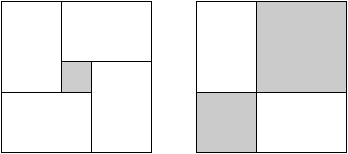
\includegraphics[scale=0.5]{FiguresMaths//FiboSquares}
        \caption{Geometric interpretation for computing $F_{n+2}^2$.}
        \label{fig:fibosquareembedded}
\end{center}
\end{figure}

Let remark that this figure might be adapted to show several properties using various decompositions of the squares and rectangles.

Another proof uses directly the definition of the Fibonacci numbers:

%$F_{n+1} + F_{n}$

$F(n+2)^2 = (F(n+1) + F(n))^2 $

$= F(n+1)^2+2.F(n+1).F(n)+F_{n}^2$

$= 4.F(n+1).F(n) - 2.F(n+1).F(n) + F(n+1)^2 + F(n)^2$

$= 4.F(n+1).F(n) + (F(n+1) - F(n))^2$

Again, using the definition of $F(n+1)$ into the square, we get the expected result:

$F(n+2)^2 = 4.F(n+1).F(n) + F(n-1)^2$
***********}


{\Arny This is another one we should discuss.  As with the section
  ``Another Identity'', Cassini's Identity does not strike me as
  ``pretty'' as the ``Consecutive products'', and the proof does not
  open the way to much new methodology.  I am troubled by Carroll's
  Puzzle because its resolution builds on principles that we do not
  cover anywhere.  Since this is not a true paradox, this material
  does not belong in that section.}


{\Arny Both of my preceding comments build on the question, Why should
  we include this material?  Obviously, when new techniques are
  involved, or when new, highly applicable, concepts are revealed,
  then the material should be included.  In other situations, I am
  just pulled by my gut feeling.  Should we discuss?}

\ignore{**************
\subsection{$\oplus$ Cassini's Identity and Carroll's Puzzle}
\label{sec:Cassini+Carroll}
\index{Fibonacci numbers!Cassini's Identity}
\index{Fibonacci numbers!Carroll's Puzzle}



\noindent \textbf{Property. (Cassini's identity)} 
\label{prop:cassini}
$F(n-1).F(n+1) = F(n)^2 + (-1)^{n+1}$ for $n \geq 1$.


The proof by induction is as follows:

\begin{itemize}
\item 
The \textbf{basis case} is straightforward since $F(0).F(2) = 2$ and $F(1)^2 +1 = 2$.

\item
The \textbf{induction step} is proved assuming the Cassini's identity holds at rank $n$.

Apply the definition of $F(n+2)$:
 
$F(n).F(n+2) = F(n) (F(n+1)+F(n)) = F(n)^2 + F(n).F(n+1)$

Replace the last term using the recurrence hypothesis:

$F(n)^2 = F(n-1).F(n+1) - (-1)^{n+1} =F(n-1).F(n+1) + (-1)^{n+2} $

Thus,
$F(n).F(n+2) = F(n).F(n+1) + F(n-1).F(n+1) + (-1)^{n+2} = F(n+1) (F(n) + F(n-1)) + (-1)^{n+2}$ 

Apply again the definition of Fibonacci sequence $F(n) + F(n-1) = F(n+1)$, we obtain:

$F(n).F(n+2) = F(n+1)^2 + (-1)^{n+2}$
\end{itemize}


The previous result (Cassini's identity) can be used for a geometrical paradox (one of the favorite puzzle of Lewis Carroll).
Consider a chess board and cut it into 4 pieces as shown in figure~\ref{paradox}, then reassemble them into a rectangle.
%Interpret this paradox.
%
\begin{figure}[htb]
\begin{center}
\label{paradox}
       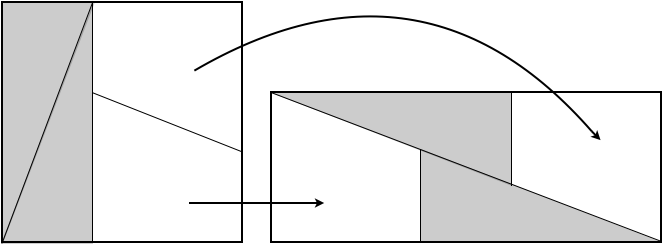
\includegraphics[scale=0.4]{FiguresMaths//FiboParadox.png}
              \caption{Construction of the rectangle after splitting the $8 \times 8$ square
              in two right $8$ by $3$ triangles and two polytopes.}
        \label{fig:FiboParadox}
\end{center}
\end{figure}

The surface of the square is $F(n)^2$ while the rectangle is $F(n+1).F(n-1)$.
In Fig.~\ref{fig:FiboParadox}, the Cassini identity is applied for $n=5$, $F(5)=8$. 
On one side, we obtain a surface of $8 \times 8 = 64$, but $13 \times 5 = 65$ on the other side!
What's wrong?

The paradox comes from the wrong representation of the diagonal of the rectangle which does not coincide with the hypothenuse
of the right triangles of sides $F(n+1)$ and $F(n-1)$.
In other words, it always remains (for any $n$) an empty space (corresponding to the unit size of the basic square of the chess board).
The greater $n$, the better the paradox because the deformation of the surface of this basic square becomes more tiny. 
***********************}

%\subsection{Using Fibonacci numbers}
%
%$F(n)$ is the number of paths from node $1$ to $n$ in the following family of graphs of figure~\ref{fibograph}. 
%
%\begin{figure}[h]
%\begin{center}
%        \includegraphics[scale=0.4]{../FIGmaths/FiboGraph.pdf}
%        \caption{Counting paths from node $1$ to node $n$ ($n=7$)}
%        \label{fibograph}
%\end{center}
%\end{figure}
%%Show how this number is related to Fibonacci's numbers.
%%\item Find a closed form for the sum of consecutive Fibonacci numbers.




%
%Figures~\ref{fig:alternatePowers2even} and~\ref{fig:alternatePowers2finalEven} illustrate the construction in the even case.
%The details are left to the readers. 
%We obtain $3.f(n)+2= 2^{n+1}$ by a similar analysis.
%However, we can deduce directly the even case from the odd case by remarking that $f(2k)=2.f(2k-1) +1$.
%
%This is obtained by the basic relations $f(n) = 2^{n} - f(n-1) -1$ and $f(2k-1) = \frac{1}{3} (2^{2k} -1)$.
%
%$n=2k$, $f(n) = 2^{2k} - \frac{1}{3} (2^{2k} -1) -1 = \frac{1}{3} (2^{n+1} -2)$.
%
%\begin{figure} [h]
%\begin{center}
%        \includegraphics[scale=0.4]{FIGmaths/alternatePowers2initEven.png}
%        \caption{Representation of the alternate series of powers of $2$ for $n=6$.
%        f(6)=32+8+2.}
%        \label{fig:alternatePowers2even}
%\end{center}
%\end{figure}
%
%
%\begin{figure} [h]
%\begin{center}
%        \includegraphics[scale=0.4]{FIGmaths/alternatePowers2even.png}
%        \caption{Case odd: Geometric proof in the odd case. Notice here that there are 2 small rectangles left at the extreme corners on the right,
%        whose surface is $1$ each.}
%        \label{fig:alternatePowers2finalEven}
%\end{center}
%\end{figure}
